\section{Plugin Eclipse}

Per il progetto è stato sviluppato un plugin per Eclipse che si occupa di:
\begin{itemize}
  \item text-highlight
  \item controllo degli errori
  \item compilazione
\end{itemize} 

Il pacchetto viene fornito sia come archivio (da estrarre nella cartella di un
eclipse) sia come IDE completo basato sul platform di Eclipse 3.2 (Callisto).

\begin{figure}[htp]
\begin{center}
  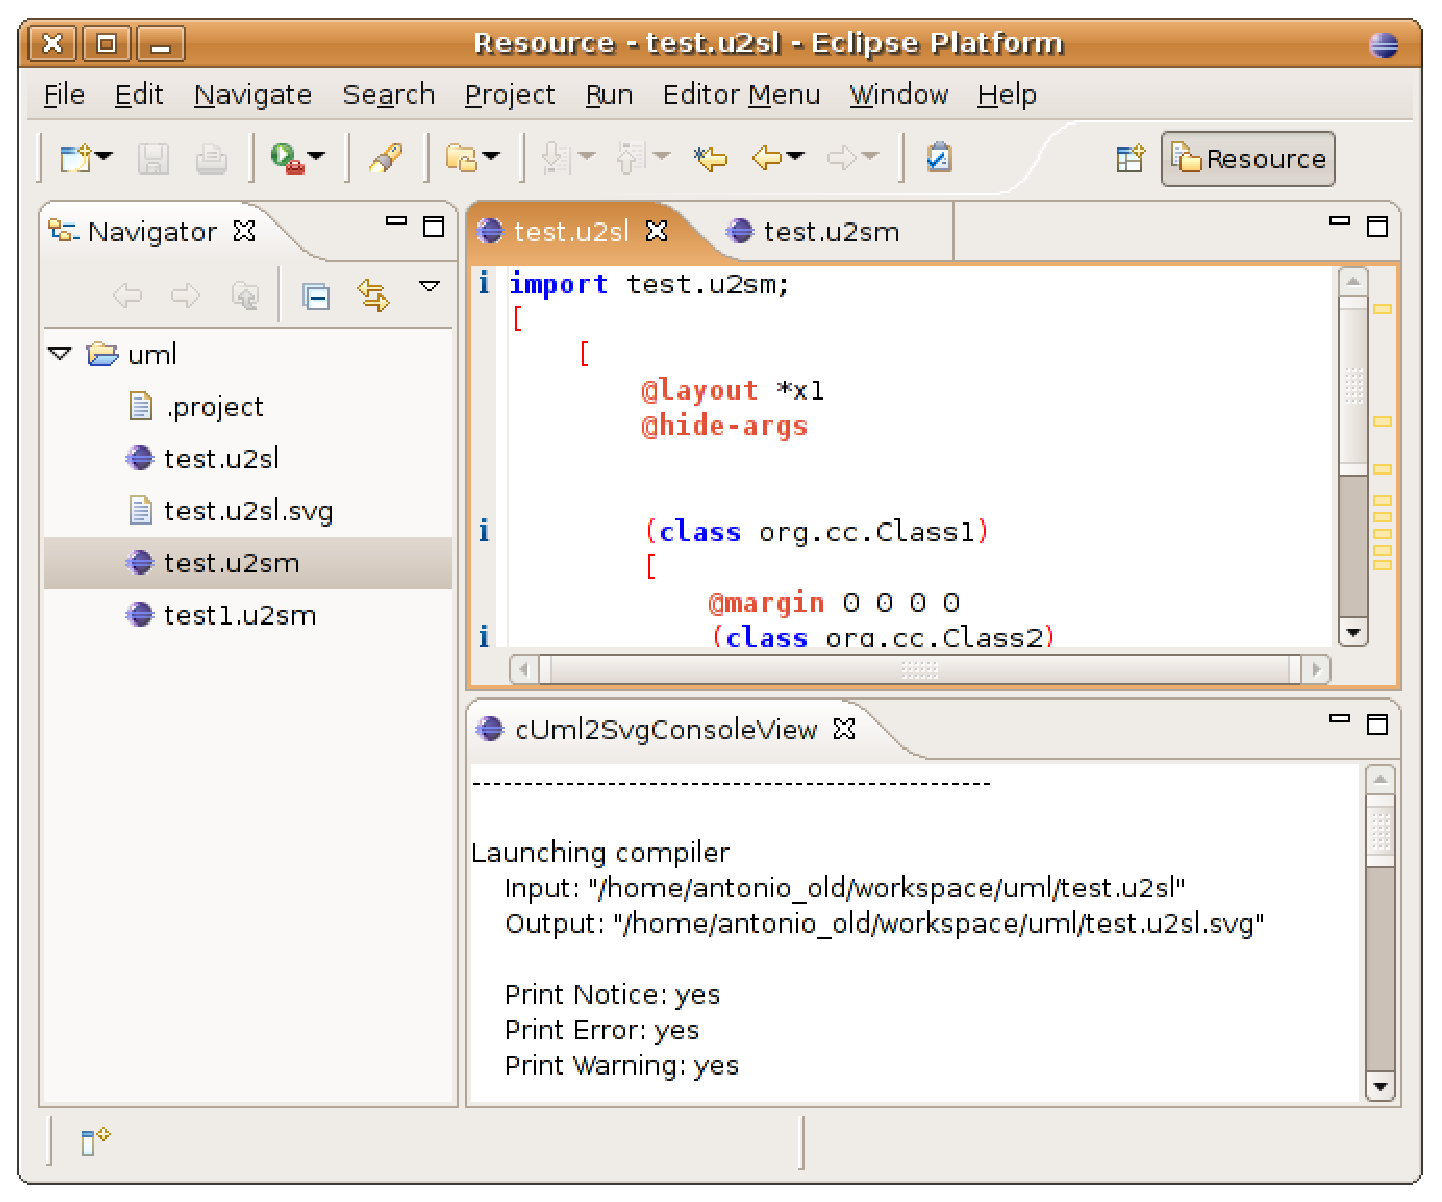
\includegraphics[width=0.9\textwidth]{img/eclipse}
  \caption[labelInTOC]{Screenshot dell'ambiente eclipse con un editor di layout
  attivo}
  \label{errorieditor} 
\end{center}
\end{figure}



